\documentclass[a4paper,dvipdfmx]{jsarticle}
\usepackage{url}
\usepackage{graphicx}
\usepackage{here}
\usepackage{amsmath}
\usepackage{float}
\usepackage{color}
\usepackage[setpagesize=false]{hyperref}
\usepackage{pxjahyper}
\usepackage{booktabs}
\usepackage{natbib}
\bibpunct[:]{(}{)}{,}{a}{}{,}
\renewcommand{\figurename}{Fig.}
\renewcommand{\tablename}{Table }

\begin{document}
\bibliographystyle{elsarticle-harv}

\title{My sample TeX file}
\author{akimanabe}
\date{}

\maketitle

\section{Introduction}
Hello World! This is my simple TeX sample documentation.

Here is what I will give you, an equation by von Bertalanffy.

\section{Materials and Methods}

Von Bertalanffy is ubiquitously used in the world of fisheries science. Here is an equation.

\begin{equation}
\label{eqn:vb}
L_t = L_\infty (1-\exp(-K(t-t_0)))
\end{equation}

\section{Result}

This is a simple schematic of von Bertalanffy trajectory which was calculated based on equation \ref{eqn:vb}.
Figure \ref{fig:vb} shows a simple growth up to asymptotic growth.
However, von Bertalanffy growth function (VBGF) was considered as not appropriate by the recent study \citep{manabe2018}.

\begin{figure}
  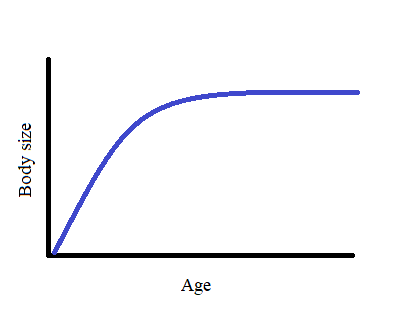
\includegraphics[width = \linewidth]{figs/samplevb.png}
  \caption{A schematic of growth trajectory by equation \ref{eqn:vb}}
  \label{fig:vb}
\end{figure}

\bibliography{refs}

\end{document}
